\documentclass{article}
\usepackage[utf8]{inputenc}
\usepackage{graphicx}
\usepackage[T1]{fontenc}
\usepackage{tabularx,ragged2e,booktabs,caption}
\usepackage{xcolor,colortbl}

\newcolumntype{C}[1]{>{\Centering}m{#1}}
\renewcommand\tabularxcolumn[1]{C{#1}}
\title{Context-Driven Virtual Overlays}
\author{Vivek Warriar}
\date {\today}
\begin{document}
\maketitle
This document outlines the project proposal for understanding how to augment contextually relevant data in Head Mounted Displays (HMDs).

\section{Augmenting Digital information} \label{Intro}
In Virtual Reality and Augmented Reality (AR) experiences (including but not limited to 360 video and hololens style applications), overlays are often used to provide additional data in a scene. Various  visual representations and interaction models could be employed to deliver this data to users. Examples of these would be (but not limited to) a heads-up display approach where information always appears in a fixed depth static container in the viewer’s field of vision or data overlays that appear around the position of the object of interest. 

In the past studies have been conducted around text representation over graphic backgrounds \cite{Jankowski:2010:ITV:1753326.1753524}, which focus on specific visual characteristics such as text placement and style on readability  \cite{Debernardis6520861,Gattullo6994851}.

Also relevant are evaluations of the impact of AR applications in various contexts and their impact on task performance. These include studies which have looked at AR applications in industrial environments \cite{Tati20171}, vehicle navigation \cite{Large:2017:ALD:3050112.3050114}, and other guided tasks \cite{Smith:2015:VST:2799250.2799291}.

Although these studies investigate the effect of text layout and style on information retention and readability they do not investigate the effect of using different interaction models on these things. I propose to address this gap in the literature. In particular I am interested in whether, allowing a user to retrieve overlay information actively rather than passively would result in improved task performance (which is a combination of information retention and performance time) and decreased mental load. I am also interested in whether object outlines (stroke) can be used to aid cognition.

The underlying theory is that if a subject's visual involvement with an object in a scene increases, the mental effort they apply on that visual stimulus would increase and the information they would retain about the object increases because in this model overlay information is only presented upon request the subject's focus of attention should be on the information itself. 

Testing this hypothesis requires an experimental study that gathers both qualitative and quantitative data from participants, details of which are described over the course of this document. I also provide a brief background on topics that are relevant to this project. 

\section{Literature Review} \label{LitReview}
This section presents some background work that has been conducted around data overlays. These studies have been grouped according to their theme of research, which are: 
\begin{itemize}
\item Annotation techniques of graphical elements
\item Representation of text in VR/AR
\item Other Relevant applications  of AR and VR
\item Attention, Memory and Mental Effort
\end{itemize}

\subsection{Annotation and Labeling techniques of graphical elements} \label{Labels}
The studies described in this section focus on methods and techniques for adding labels and annotations to graphical elements. The primary applications of these techniques is to enhance the learning and understanding of technical images and 3D models.

Mayer \cite{mayer2002multimedia} presents the theory of Spatial Contiguity which shows that the effectiveness of text explanations does not depend only on the contents of the text. Another important factor for learning is the location of the text in relation to the image it is describing. According to Mayer the nearer the text is placed to the image, the more improved the learning. This is because readers do not waste mental effort is moving between the text and the image. Spatial proximity also allows readers to hold both text and images in their working memory and allow them to make better inferences between the two \cite{mayer2002multimedia}. 

A focus of work in this field has been to create algorithms that effectively deal with label placement around graphics.For 2D non-interactive graphics Hartmann et al \cite{Hartmann2004} present an approach using dynamic potential fields which calculate attractive or repulsive forces between textual and graphical elements to generate label layouts. 
The authors in a follow-up study \cite{Hartmann2005b} analyze a large amount of hand drawn/annotated illustrations and present metrics for aesthetic label layouts. They concluded that aesthetic choices of layouts largely depended on individual preference, they also present an algorithm that calculates these label layouts taking into account user preferences as one of the weights for the the label placement around non-interactive graphics. 

In theory it would be possible to use this technique to generate test material that takes into account an individual user's aesthetic preferences and thus minimize the effect of this factor on test. I could use this technique to generate test material which would minimize the impact of user preference, however for this initial study I do not propose to do this.

Similarly Ali et al\cite{ali2005label} present an algorithm to ensure label layout coherency between frames for interactive animated graphics. This means for example if text or graphics are being scaled in response to user interaction, the position and layout of all the elements remain coherent. Another approach to frame coherency is using what Götzelmann et al define as \textit{local agents} i.e "local strategies to optimize the layout and to minimize the flow of layout elements in subsequent frames"\cite{Gotzelmann2006}. 

Ritter et al \cite{Ritter:2003:ISI:604045.604072} present a technique for the interactive exploration of graphics and models with multiple (2d and 3D) views. They use the metaphor of shadows to link the spatial (3D) and non-spatial (2D) views and dynamically annotate information about the views as the user explores the graphics. Figure 1 shows an example of the \textit{Illustrative Shadows} approach. 
\begin{center}
	\begin{figure}[!ht]
    \vspace{1cm}
		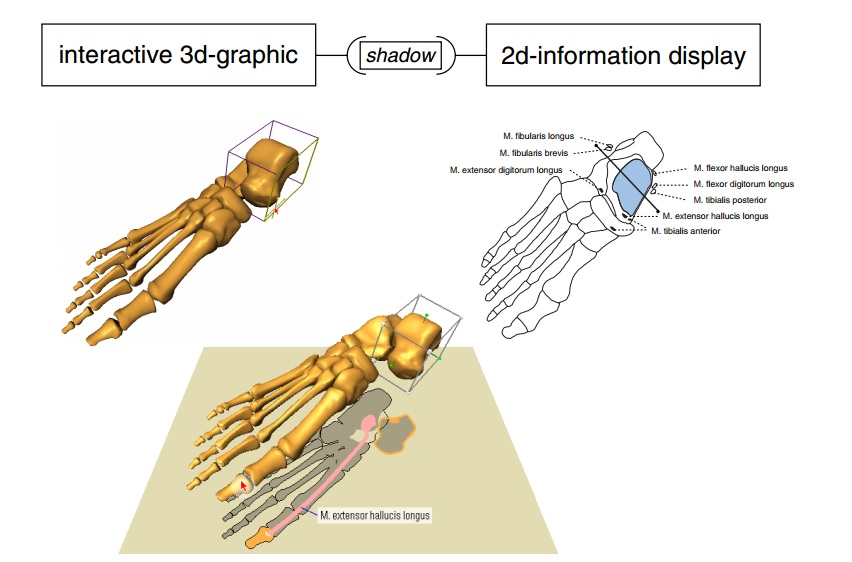
\includegraphics[width=\textwidth]{Images/illustrativeShadows.jpg}
    	\caption{Illustrative Shadows by Ritter et al \cite{Ritter:2003:ISI:604045.604072}}
        \vspace{1cm}
    \end{figure}
\end{center}

\textit{Zoom Illustrations} is a technique created by Preim et al \cite{preim1997coherent} which was developed for the exploration of 3D models. It uses the concept of fish-eye views to emphasize aspects of the model that the user is focusing on. This technique involves dynamically modifying the geometry of the model and scaling up objects of interest and scaling down other objects. Figure 2 shows an application of Zoom Illustrations.
\begin{center}
	\begin{figure}[htbp]
    \hspace{0.1\textwidth}
		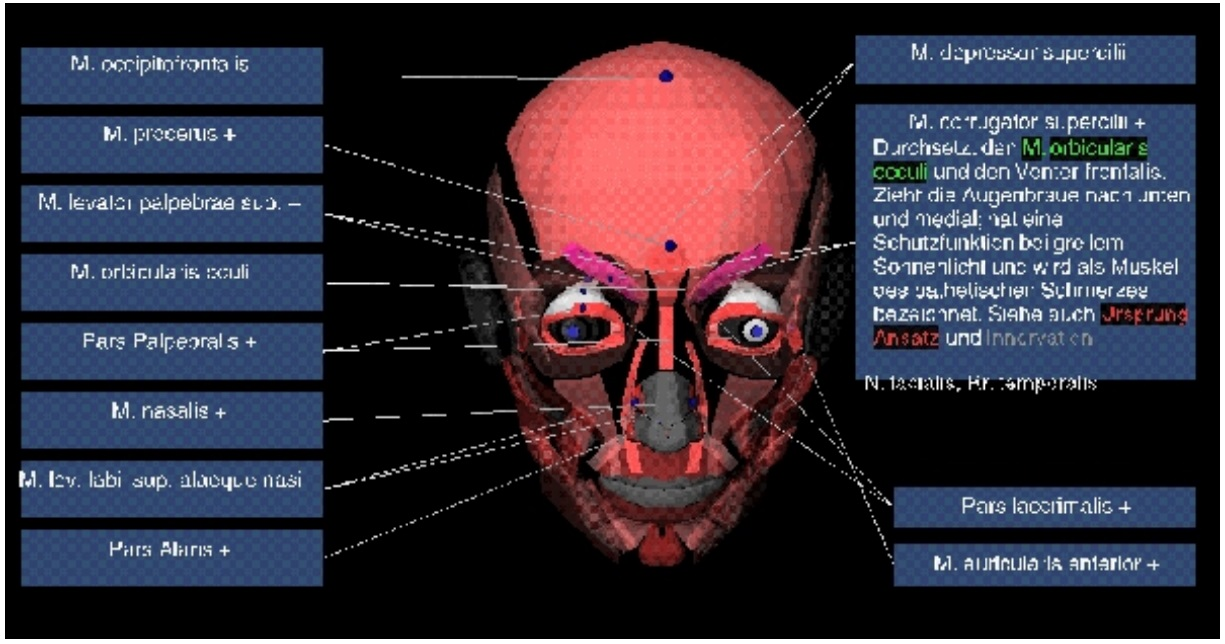
\includegraphics[width=0.8\textwidth]{Images/zoomIllustrations.jpg}
    	\caption{\textit{Zoom Illustrations}: One muscle (above the eyes) has been enlarged to be explained, it's corresponding text box has been expanded while other muscles and text boxes have been scaled down and moved
away \cite{preim1997coherent}}
    \end{figure}
\end{center}
Chigona and Strothotte \cite{Chigona:2002:CTE:569005.569010} describe an approach known as the\textit{Dual-Use of Image Space (DUIS)} for text explanations of non-photo realistic illustrations. Here the pixels for the text explanation have also been used for the shading in the illustrations. They argue that this approach would allow users to compare information with minimum cognitive effort, as well as providing efficient use of screen real estate. Figure 3 shows an application of \textit{DUIS}. 

	\begin{figure}[htbp]
		\hspace*{2cm}
        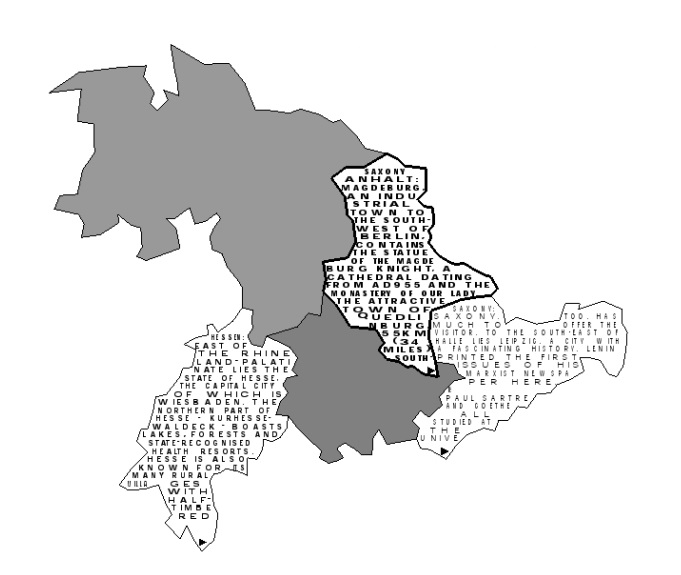
\includegraphics[scale=0.35]{Images/duis.jpg}
    	\caption{\textit{DUIS} by Chigona and Strothotte \cite{Chigona:2002:CTE:569005.569010}}
    \end{figure}

Sonnet et al \cite{Sonnet:2004:IEA:989863.989871} present a technique for interacting with 3D models where dynamic explosion diagrams of the models are created allowing users to explore parts of the 3D model that are occluded from view. This technique is mouse driven and allows for scrollable text annotations to be loaded as a user's exploration triggers areas of the model. The advantage of this technique is that it provides textual content within the spatial context of the 3D diagram, in this way it overcomes occlusion issues. Figure 4 illustrates the explosion probe technique.

\begin{figure}[htbp]
		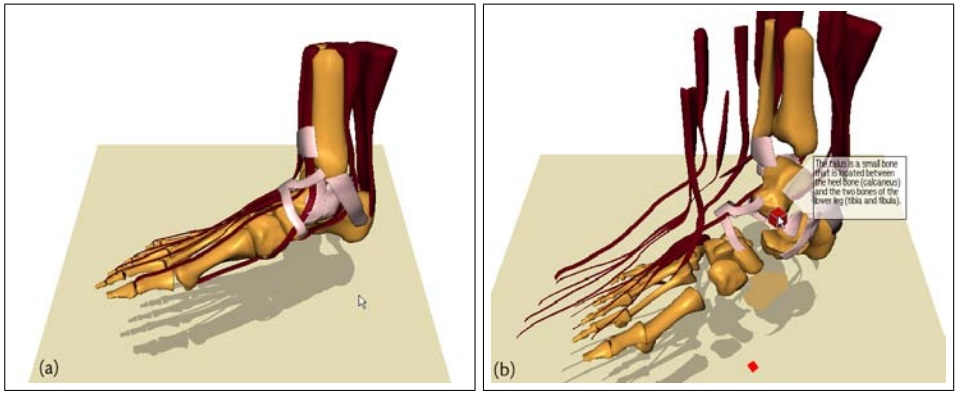
\includegraphics[width=\textwidth]{Images/explosion.jpg}
    	\caption{\textit{Explosion Probe}: (a) Anatomical diagram of a foot and (b) explosion diagram with an interior bone labeled.\cite{Sonnet:2004:IEA:989863.989871}}
    \end{figure}

From these studies we can see that annotating graphics with text is a complicated subject with multiple possible approaches. Sonnet et al in a later study compared the impact that different annotation techniques have on the comprehension that a particular text annotation and it's relation to a particular graphical element, as well as the comprehensibility of  the text during exploration \cite{Sonnet2005}. The various techniques compared were:
\begin{itemize}
\item attaching the text directly to the object
\item placing the text in the object’s shadow
\item using symbols to make the correlation between the object and the text
\item using a line to make the visual connection from the text to the object with and without additional hints in the shadow
\end{itemize}
Their study indicated that there was no one particular technique which was better than the others. Each technique had advantages over the others depending on context. For example when working with short labels, attaching the label close to the object using a visual connection (connection line) seems to work well and was preferred by participants in the study.

The studies mentioned here are important to my proposed experiment as most of these techniques could be adapted to work with annotations in 360 video and AR applications. However, one of the main considerations is that these annotation techniques have been designed for illustrations and 3D graphics that are not integrated into a 360 view. Techniques such as the dynamic potential fields labeling \cite{Hartmann2004} and user preference based placement \cite{Hartmann2005b} could potentially occlude other objects of interest within a heavily populated 360 environment whereas they are less problematic in, for example, a text book where a specific areas are reserved for graphical illustrations. 

Another consideration is that these techniques are not designed for mixed reality experiences. For instance techniques like \textit{Illustrative Shadows}\cite{Ritter:2003:ISI:604045.604072}, \textit{Zoom Illustrations}\cite{preim1997coherent}, \textit{DUIS}\cite{Chigona:2002:CTE:569005.569010} and the \textit{Explosion Probe}\cite{Sonnet:2004:IEA:989863.989871} would potentially be computationally expensive to bring into an AR or VR experience.  

Also a review of the studies in this section reveals a useful taxonomy for describing annotations. Labels can be of two kinds, external and internal. External labels require child elements such as connecting lines and anchor points between themselves and the reference object, and internal labels are overlayed on the reference object. Also more comprehensive labels are referred to as annotation boxed and these can contain both text and graphic media.

\subsection{Representation of text in VR and AR}
This section explores the representation of text in AR and VR experiences. Most of these studies focus on ensuring readability by varying the text style as required for different environments, devices, backgrounds. 

Jankowski et al \cite{Jankowski:2010:ITV:1753326.1753524} explored how text would be incorporated with Video and 3D graphics. They compared image polarity (bright images with dark text and vice versa), text style (plain, billboard, anti-interference, text shadow) and background style (video and 3D) on reading performance. Results from the study indicated that there was very little performance difference between video and 3D conditions, negative polarity (dark image and light text) showed a higher performance and  billboard out performed the other text styles.Billboard was also preferred the most by participants in the study. Although it is not a context specific approach, their study could potentially inform the text style for VR and AR experiences as well. Figure 5  shows the difference text styles used in the experiment design. 

\begin{figure}[htbp]
		\hspace*{0.15\textwidth}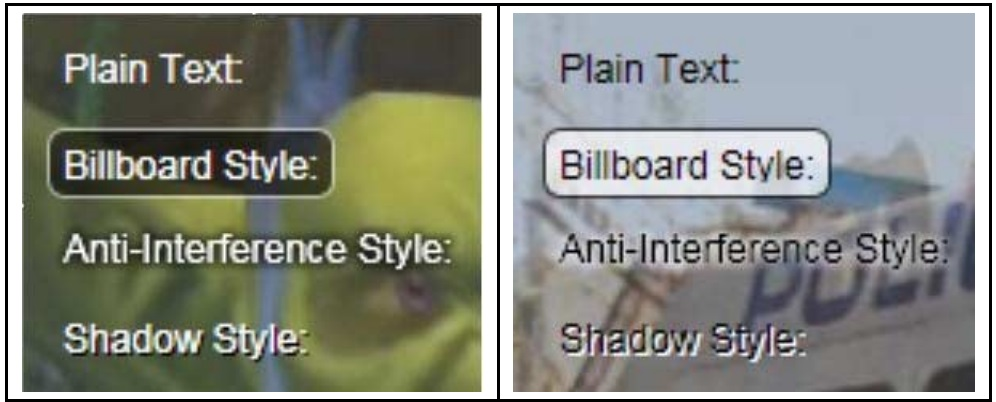
\includegraphics[width=0.8\textwidth]{Images/textStyles.jpg}
    	\caption{Various text styles for overlaying text on video (right: negative polarity, left: positive polarity)\cite{Jankowski:2010:ITV:1753326.1753524}}
\end{figure}

In earlier work, a subset of the authors \cite{Jankowski:2009:FGC:1559764.1559793} present a system \textit{2Lip} which is a two layer interface operating in a 3D environment. Interface elements within the 3D environment can be clicked to call up a large body of explanatory text that appears as a translucent zero-depth overlay. They apply it in a visual encyclopedia where the 3D environment still visible behind the overlay text which describes it. 2Lip is a web browsing interface and users navigate through both layers using hyper-links in the text layer of the interface. The study conducted shows that the interface has a positive effect on visual and associative memory. Figure 6 shows a screen-shot of the 2Lip interface used in their study.  
\begin{figure}[htbp]
		\hspace{0.2\textwidth}
        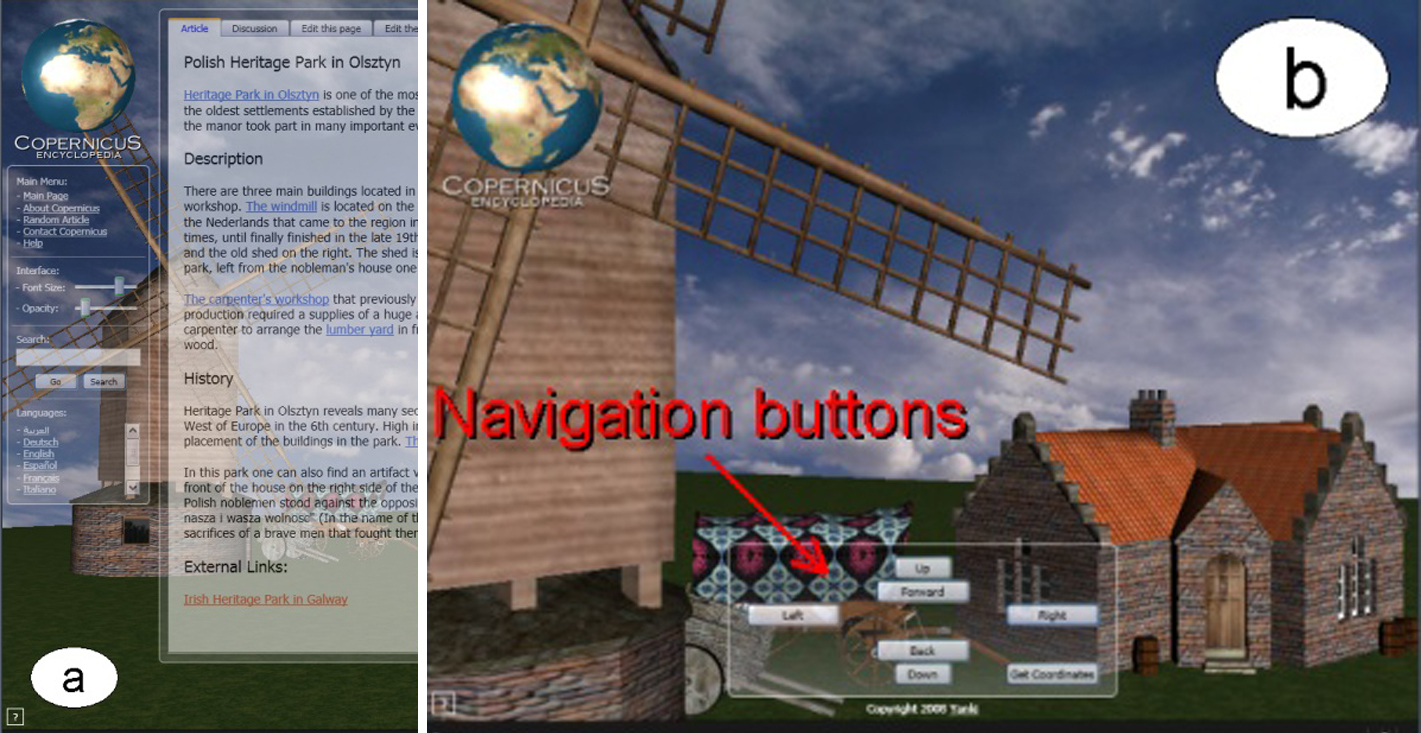
\includegraphics[width=0.6\textwidth]{Images/2lipv2.jpg}
    	\caption{\textit{2Lip} interface, (a) article view; (b) navigation view  \cite{Jankowski:2009:FGC:1559764.1559793}}
\end{figure}

Maass and Döllner present two techniques for dynamic label placement in virtual space \cite{Maass2006,Maass:2007:ELL:1294685.1294695}. The first technique treats the labels as 2.5 dimensional elements and places them according to the available space in the viewing plane. The technique aims to prevent occlusion of labels however, in situations where that is not possible, the label that is closer to the viewer is given prominence. This technique is useful for describing specific objects of interest within a scene. Figure 7 shows the application of this technique. 
\begin{figure}[htbp]
		\hspace{0.2\textwidth}
        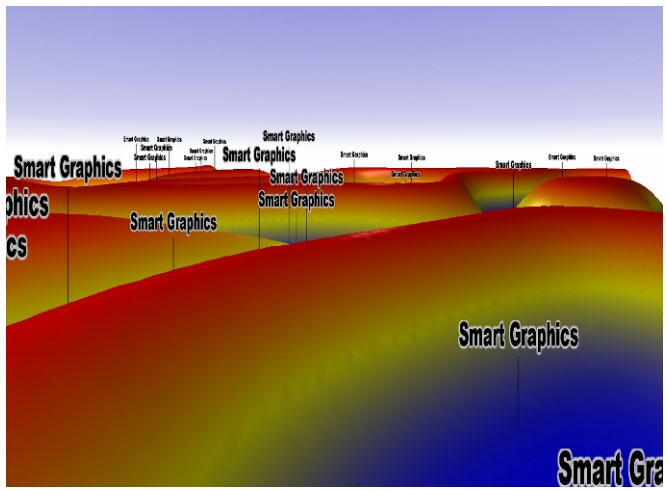
\includegraphics[width=0.6\textwidth]{Images/labelplacement.jpg}
    	\caption{Label placement using simulated height and depth in a representation of a 3D landscape\cite{Maass2006}}
\end{figure}

The second technique places the label over the surface of the labeled object. These embedded labels ensure a "high correlation between label and annotated object", minimize the possibility of occlusion and efficiently utilize screen real estate \cite{Maass:2007:ELL:1294685.1294695}. This technique would potentially be useful to annotate objects with flat surfaces or line features such as roads. It would not work for annotating objects with complex surfaces like a human being. Figure 8 shows the application of this technique to a virtual city. 

\begin{figure}[htbp]
		\hspace{0.175\textwidth}
        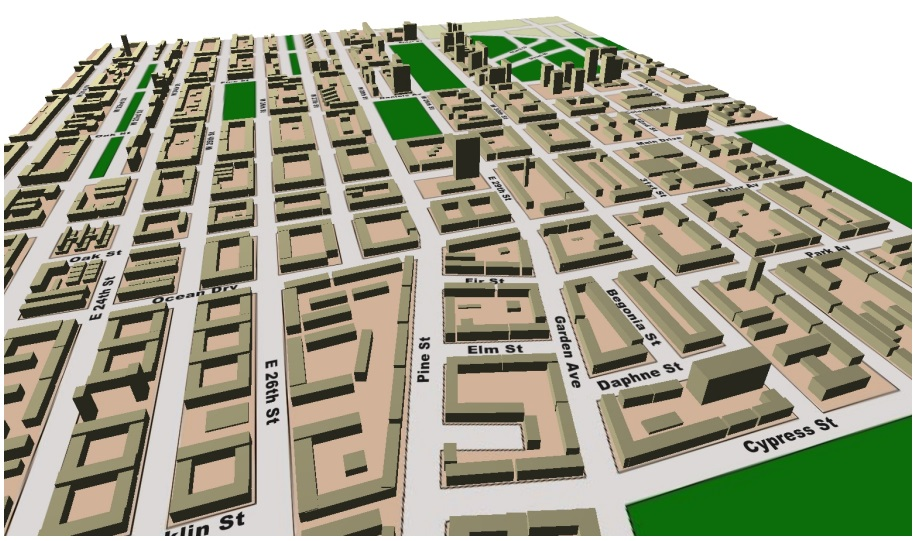
\includegraphics[width=0.65\textwidth]{Images/embeddedLabels.jpg}
    	\caption{Embedded Labels  in a 3D virtual city \cite{Maass:2007:ELL:1294685.1294695}}
\end{figure}

Vaaraniemi et al introduce two more techniques through their work in annotation of roads in navigation systems \cite{Vaaraniemi2013}. The aim of these approaches is to allow a features which would otherwise be occluded (for example roads which would be occluded by buildings or other structures) to be made visible in some way. The first approach uses 'Transparent Auras' to allow a feature's label to 'shine through' an object which is occluding it. The second approach allows the entire feature which is being occluded to 'glow' through the areas that are occluding it. These approaches allow us to label 'hidden features' in an environment. In user testing both approaches performed significantly better than simply drawing labels over occluded objects. These techniques could potentially be transferable to 360 video and story telling. However, their adaptability to AR maybe limited where environment information is limited. Figure 9 shows the application of these techniques.  

\begin{figure}[htbp]
		
        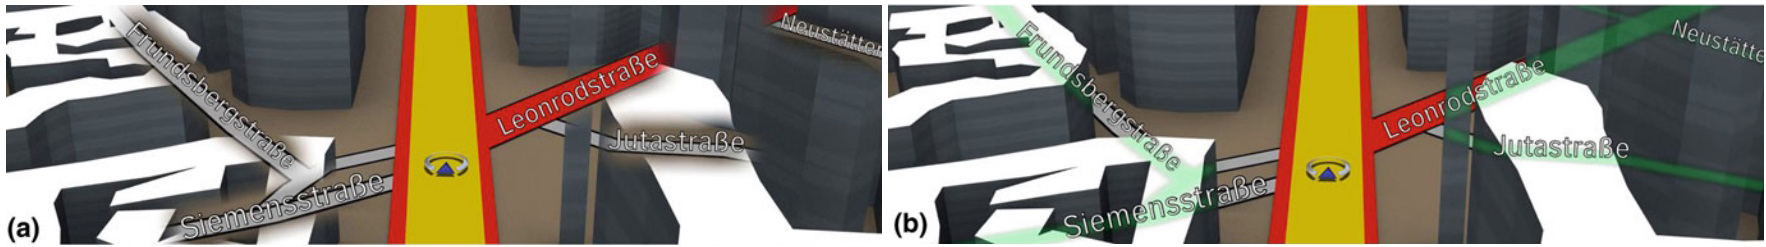
\includegraphics[width=\textwidth]{Images/navigationv2.jpg}
    	\caption{(a) Technique using transparent auras (b) Technique using glowing roads \cite{Vaaraniemi2013}}
\end{figure}

Grasset et al \cite{Grasset6402555} describe methods of annotation for augmented reality browsers where there is limited environment information. Their approach is image based where the layout of the labels is dependent on the underlying scene being annotated over. This approach involves analyzing the saliency map of the image being viewed, (which is an indicator of how busy the image is) and using edge detection to reveal objects in the image. This information is used to place labels in areas of low saliency and also ensures that labels do not occlude edges in the scene. Also the color of the image background is used to optimize the color of the connection lines and of the background of the label to ensure maximum readability. This approach is very relevant to the treatment of annotations in augmented reality experiences. However, the authors acknowledge that the solution is not applicable in a scene of very high saliency. It is also worth noting that these techniques have been created for mobile devices, do not target HMDs specifically. Figure 10 shows the applications of these techniques as compared to naive approaches. 

\begin{figure}[htbp]
		\hspace{0.075\textwidth}
        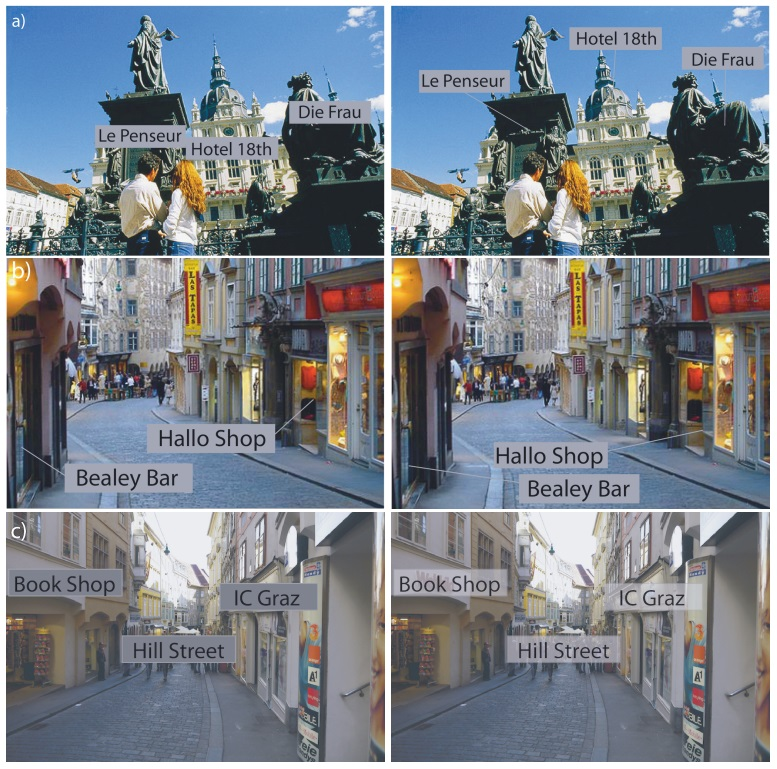
\includegraphics[width=0.85\textwidth]{Images/imageBased.jpg}
    	\caption{ Illustration of three of three real world considerations (from top to bottom), bad (Left) and good (Right) examples of: (a) avoiding overlap on salient areas, (b) avoiding overlap on edges, (c) improving contrast between video image and labels \cite{Grasset6402555}
}
\end{figure}

As I will be using head mounted display devices in my experiment, it is important to highlight a study conducted by Debernardis et al \cite{Debernardis6520861} which compared text readability in video see-through versus optical see-through HMDs. \textit{Video See-Through (VST)} devices are commonly used for virtual reality at present (the Occulus Rift is an example of a VST HMD) . \textit{Optical See-Thorugh (OST)} devices are ones which are generally associated with Augmented Reality Experiences (the Microsoft HoloLens is an example of an OST HMD). The results of the study indicates that readability is considerably affected by the type of HMD used. Readability was faster on OSTs. Using VSTs it was found that the background did affect readability but only when text was used without a billboard. Debernardis et al recommend a good text style for both HMDs is white text on blue billboards, referring to RGB (0,0,255) which was the color they used in the experimental set up. 

In a follow up study Gattullo et al  \cite{Gattullo6994851} investigated the effect of text outlines and contrast polarity on text readability using both VST and OST HMD devices in different lighting situations (to simulate use in industrial environments). The study found that in high illuminance lighting conditions VSTs performed better than OSTs regardless of contrast polarity and text outline width. The study also revealed that in negative contrast polarity (light text on dark background) VSTs were preferred with a text outline of a minimum of 1px causing an improvement in readability. In positive contrast polarity (dark text on light background), OSTs were preferred and a text outline gave no improvement. 

In Gattullo et al's investigation into the use of HMDs in industrial contexts, the authors explored the effects of different text style and colors on readability \cite{Gattullo7064667}. Results of the study show that either outline or billboard text styles are effective for text legibility. A colored billboard with white (or neutral) text was most effective. When color coding is not required, the authors recommend using a blue billboard along with white text. 

Under the canopy of text readability studies that focus on industrial applications, Fiorentino et al \cite{fiorentino2013augmented} conducted a study exploring the effect of the background and text style on readability using an OST HMD.  The study shows that both factors influence text readability. What is interesting about the study it that the authors report that "that presentation mode of the text has a differential effect on task completion time and error rate", meaning that presentation modes are preferred for completion time and error rate are different from each other. This shows that depending on the priority of the task (fast reading or high accuracy), different presentation modes would have to be selected. 

As we have seen so far the studies that explore text readability in HMDs focus primarily on text style. The work by Orlosky et al \cite{6671805,Orlosky:2013:DTM:2449396.2449443,Orlosky:2014:MMT:2636242.2636246} takes a slightly different approach. The research addresses placement or location of text in OST HMDs to maximize readability and environment awareness, but the authors take an 'intelligent view management' approach, using camera tracking to analyze dark and reduced salient areas of the users field of view in order to place text in that location. It is worth noting that their system mimics human tendencies of text placement. As part of the development process, a study was conducted where participants placed text on videos. This enabled the creation of a system that closely mimics human preferences of text placement in the subject's field of view. The focus of this work has been on migrating user centric-content like sms, email, social media updates to HMDs. 

Since the work focuses on visualizing text data that is external to the scene, it remains to be seen whether it also can be applied to the placement of text data that describes objects in a scene. For example the work by Orlosky et al allows text data to be moved to different areas of the scene depending on the availability of dark and 'uncluttered' areas of the view, however when we consider text that is being  used to label an object in a scene it maybe beneficial for the label to remain fixed in it's location and as close as possible to the object it refers to. The techniques described in Orlosky et al \cite{Orlosky:2014:MMT:2636242.2636246}  may need to be adapted for the use cases I am investigating, further research is advised.

From the studies reported in this subsection it is possible to compile guidelines for representation of text style in HMDs for good readability. These studies for the most part do not address the issues with occlusion (labels occluding scene objects and  other labels), especially in scenes with high saliency \cite{Grasset6402555}. 

Another gap in existing knowledge is the lack of interaction models for retrieving information about objects within a scene viewed with HMDs. Since the studies that have explored contextualized text (text related to the scene being viewed) have been within industrial applications, the results may change when applied to non-industrial applications for example location specific content, story telling or other consumer centric applications. This is because designing for industrial environments assumes the user to have had a certain amount of training and domain awareness and the content itself is more instructional in nature, these assumptions cannot be made in non-industrial contexts. 

\subsection{Other Relevant Research}
This section reviews related research in the AR and VR space which the my study would contribute to. 

Santos et al \cite{SousaSantos2008} compared the user performance between a HMD and a desktop where the user performed a navigation task in a game scenario. The results indicate that although participants found the HMD experience acceptable and described the interaction as intuitive, they performed significantly better in the desktop condition of the experiment. This study shows that user performance changes between a screen and a HMD experience. This indicates that some of the results from previous screen based research \cite{Grasset6402555} may suffer a performance drop in a HMD environment. 


Salomoni et al \cite{Salomoni2017} introduce the concept of diegetic interfaces. These are GUI components designed to be interacted with in a natural way to enhance the immersion of the experience. These interfaces use hand tracking to enable the user to press virtual buttons and interact with virtual components. Figure 11 shows an example of a diegetic interface along with it's non-diegetic counterpart. These interfaces may enable higher immersion however, an argument could be raised about the applicability of this technique across a range of HMDs, since not all HMDs have hand tracking capabilities. Also the current low resolution of existing HMDs affects this technique for example an appropriate diegetic interface may created on pre-existing elements in the virtual environment e.g signs and posters, however if the resolution of these elements is too low it would be impossible to place an interface onto them. 

\begin{figure}[htbp]
		\hspace{0.15\textwidth}
        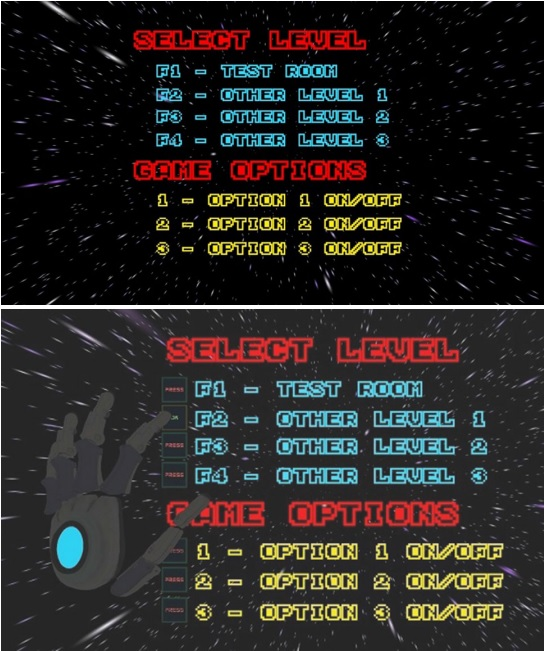
\includegraphics[width=0.7\textwidth]{Images/digetic.jpg}
    	\caption{ Above: Non-diegetic interface; Below: Diegetic Interface \cite{Salomoni2017}
}
\end{figure}

In my experiment I propose to investigate the use of information overlayed onto lifelike scenes/environment using captured 360 video. I will implement gaze interactions to trigger information objects. Müller and Dauenhauer \cite{Mller2016} present a taxonomy for linking information in augmented reality. This taxonomy is intended to facilitate analysis for visualizations similar to the ones I will use in my experiment. Their taxonomy breaks up visualizations into parent and child elements, these are: spatial anchor, information object, and information connection. There are also three corresponding dimensions of evaluation which are: reference system, visual system and context. This taxonomy is highly relevant to my proposed study as the proposed experiment will investigate the effect of an interaction model where spatial anchors are used to trigger information objects. Here, spatial anchors would be objects in a scene and the information objects would be the corresponding annotation-containing information about the spatial anchor. I will also explore the effect of strokes around these spatial anchors on a viewer's cognitive information processing. 

It is worth noting that Müller and Dauenhauer also explored different types of visual connections between spatial anchors and information objects. The different conditions of their experiment were: spatially assigned, continuously connected (with lines), symbolically connected with color and symbolically connected with shape. Figure 12 shows  the different conditions of the experiment. The results indicate that linking information close to the spatial anchor gave the best task performance followed by information connection using connection lines.  

\begin{figure}[htbp]
		\hspace{0.2\textwidth}
        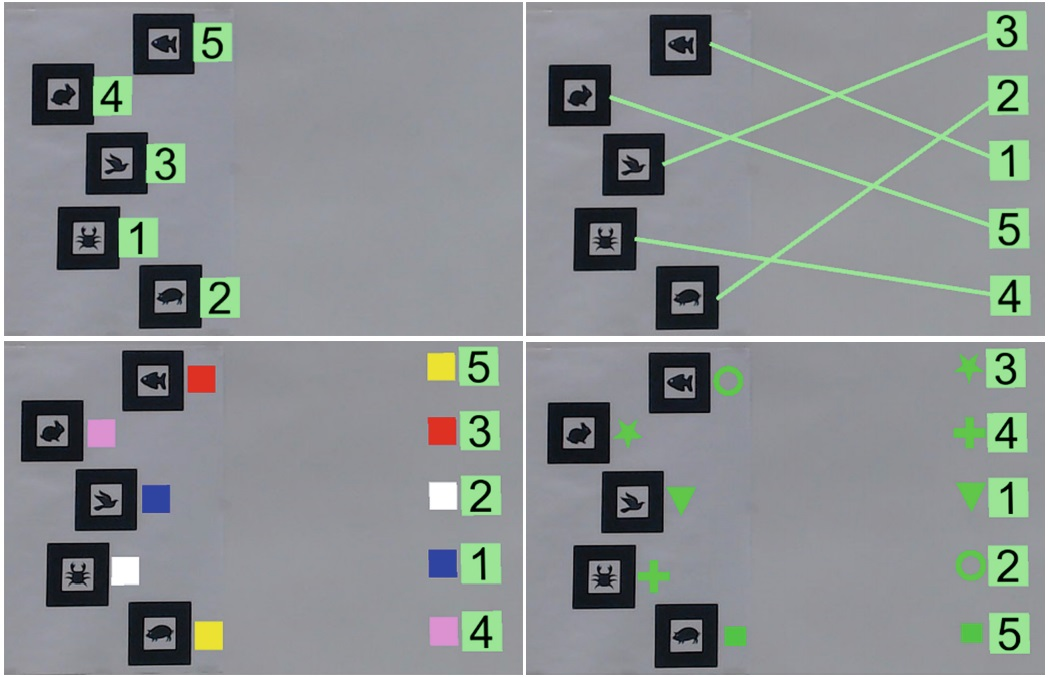
\includegraphics[width=0.6\textwidth]{Images/infoLink.jpg}
    	\caption{The different conditions in the study conducted by Müller and Dauenhauer. Top-Left: Spatially assigned; Top-Right: continuously connected; Bottom-Left: Symbolically connected with color; Bottom-Right: Symbolically connected with shape \cite{Mller2016}
}
\end{figure}

In a follow up study, the authors investigate the effects of occlusion in 3D scenes on task performance \cite{Mller7836504}. The different conditions being compared were: an incorrect occlusion scenario where connection lines where never occluded, a correct occlusion scenario where lines were occluded partially depending on the location of the spatial anchor in 3D space, and a condition using symbolical connections using color. Figure 13 shows the different experimental conditions used. The results from the study indicate that partially occluded connections were most preferred and that the interference in the connection lines did not have any effect on task performance.  

\begin{figure}[htbp]
		
        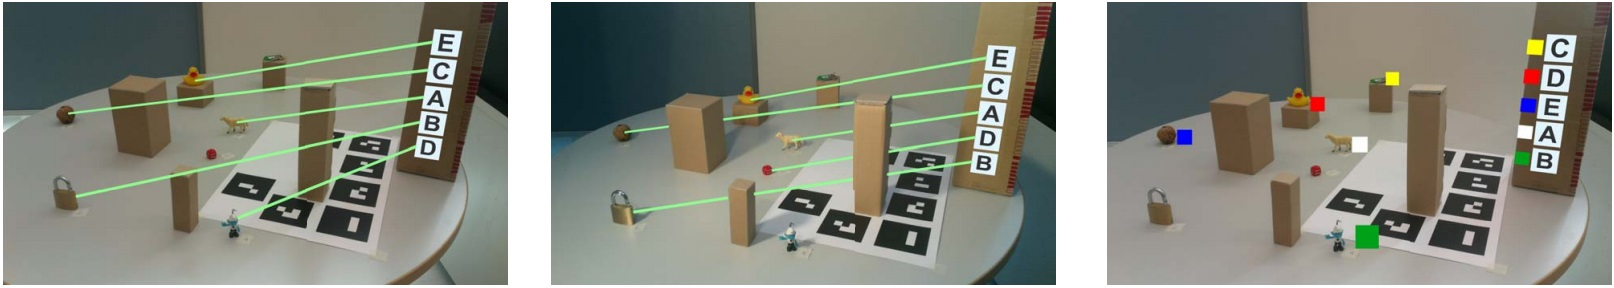
\includegraphics[width=\textwidth]{Images/occludedLink.jpg}
    	\caption{The different conditions in the second study conducted by Dauenhauer and Müller. Left: Condition with incorrect occlusion; Middle: condition with correct occlusion; Right: condition
with color connections \cite{Mller7836504}
}
\end{figure}

Seigl et al \cite{Siegl20071895} describe a system for "3D augmented pointing, which combines inside-out tracking for head pose recovery and 3D stereo human–computer interaction."  Experimental evaluation showed that the "accuracy of this 3D cursor is within a few centimeters, which is sufficient to point at an object in an office." However the study did not compare the use of the 3D cursor to other pointing mechanisms such as gaze.  Interestingly however, the authors also propose a software model describing a mechanism for active memory and learning which could be relevant in creating an AR system which uses newer technologies for example gestural interfaces. 

The studies reviewed in this subsection are meant to provide context to the proposed study. The study is built upon the study conducted by Müller and Dauenhauer \cite{Mller2016} and could potentially be integrated with the work conducted by Seigl et al \cite{Siegl20071895}. 

\subsection{Attention, Memory and Mental Effort}
In previous sections of this document I have reviewed applications of different styles of text overlays in VR and AR. The objective my study will be to measure the impact of the proposed interaction model on mental effort investment, task performance and information retention. This section therefore reviews some of the work regarding aspects of human cognition relevant to my study. 

Baddeley and Hitch \cite{baddeley1974working} propose a model of working memory (which builds on Atkinson’s and Shiffrin’s multi-store model \cite{atkinson1968human}) to explain cognitive information processing. According to their model, there are multiple stores in human memory which process cognitive information. Sensory input is constantly stored and updated in the sensory store. The retention time of information in the sensory store is very short and information will be discarded from this store after a few milliseconds. The process of attention acts upon this information and moves it to the working memory store which Baddelay and Hitch propose is made up of multiple subcomponents. The retention time for information in the working memory store is considerably longer than the sensory store however, it is still only a few seconds. The process of rehearsal moves this information into the long-term memory store, which can hold information for very long periods of time (minutes to years). The process of recall activates information in long-term memory and moves it into working memory. Figure 14 shows a diagrams of how these stores interact with each other. This is broadly referred to as cognitive information processing.  

\begin{figure}[htbp]
		
        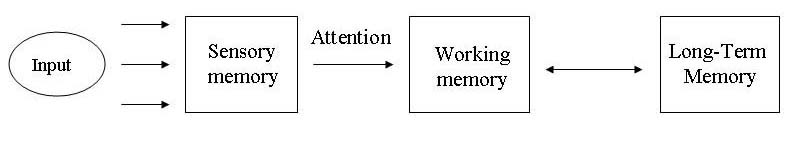
\includegraphics[width=\textwidth]{Images/workMem.jpg}
    	\caption{The working memory model proposed by Baddeley and Hitch \cite{baddeley1974working}
}
\end{figure}

Cowan \cite{cowan1999embedded} presents a contradictory view of information processing with his Embedded Processes Model. He argues that working memory is not a separate memory store but a part of activated long-term memory which he describes as the "focus of attention". This model "integrates attention, working memory and long term memory into one unitary system". Schweppe and Rummer \cite{Schweppe2014} argue for the incorporation of Cowan's work into multimedia learning.  

The study I propose will aim to analyze the effect of active vs passive data overlays on attention and cognitive information processing. I aim to interpret the results acquired using both Cowan and Baddelay \& Hitch's conflicting models. If my interaction model has an impact on information retention processes it could prove aspects of Cowan's embedded processes model, since it shows that that interacting with information alters our "focus of attention" and has an impact on the efficiency with which this information is encoded in our long-term memory. 

Alternatively if my interaction model does not have any impact in information encoding within long term memory it would prove the working memory model proposed by Baddeley and Hitch \cite{baddeley1974working} as information moves through different memory stores. The differences in attention will not have an impact on information encoded into long term memory. 

Sweller's \textit{Cognitive Load Theory} states that learning best occurs in situations where information aligns with human cognitive architectures \cite{sweller1999cognitive}. According to Cognitive Load Theory \cite{sweller1999cognitive} and Multimedia Learning Theory \cite{mayer2002multimedia} visual cues that "guide attention to the relevant elements of the material or highlight the organization of the essential material" improve the learning outcomes of multimedia instructions, this is referred to as \textit{the cuing effect} \cite{van201411}. 

A study conducted by Tabbers et al \cite{tabbers2004multimedia} proved the validity of the cuing effect when learning outcomes were higher when visual cues were added to pictures. However, there are many different forms of cues including but not limited to picture based cues, text based cues, and cues integrating text with picture elements.

Fairclough \cite{fairclough2011psychophysiological} describes mental effort as being compensatory in nature. Mental effort is the cognitive response to changing task demand such as increased working memory load, sustained task activity, environmental stressors or changes in sensory stimuli. 

The investment of mental effort will improve or sustain cognitive performance \cite{pashler1998psychology}. This is further explained by Eysnek \cite{eysenck2014anxiety} who describes "the efficiency of performance as the relationship between covert effort investment and overt performance quality" \cite{fairclough2011psychophysiological}.  

Mental Effort is of significance to this study as it is possible that different interaction models require different amounts of mental effort investment and would therefore impact task performance. Mental effort has also been shown to have an effect on information retention and learning outcomes. A study conducted by Salomon \cite{salomon1984television} compared learning from TV and reading. The results indicate that mental effort was higher for the reading condition and the increased mental effort resulted in stronger learning outcomes in terms of inference making. 

Previous research activities have proposed a number of methods to measure mental effort investment. Heart Period Variability  \cite{Lajos} and Heart Rate Variability \cite{Rowe:1998:HRV:274644.274709} are two techniques that use heart rate sensors that measure mental effort or task load. Another popular tool for measuring task load is the NASA-TLX (Task Load Index) \cite{HART1988139} which is a multi-scale questionnaire that has proven reliable over the last three decades. Originally developed for measuring workload in aviation tasks it has grown in popularity and is used to measure workload in a variety of fields \cite{Hartdoi:10.1177/154193120605000909}. 

These mental effort measurement techniques are commonly used in Human Computer Interaction research. I intend to use the NASA-TLX as it is a non-intrusive method of measuring the mental load in my study.

\section{Approach and Hypothesis of Proposed Study} \label{Approach}

My underlying assumption is that the act of consciously retrieving data about the environment increases the mental effort investment that viewers employ though this interaction.  This increase in mental effort would focus the user’s attention on the desired stimuli and increase the likelihood that the information (in my case text information from an overlay) would be retained in the user’s memory stores.

There are two variables that would be explored by my study: User Driven Information Retrieval and Object Outline Cues (Strokes) around objects with associated data.

\subsection{Information Retrieval}
The study aims to explore the impact of user drive information retrieval on information retention and task performance. This would be measured by comparing a condition where overlays about an object are always visible to the viewer and another condition where overlays become active only when a user's gaze is on the object. Figure 15 shows an example view of the condition where information overlays are always active (non-retrieval condition). Figure 16 shows an example view where information is activated when a viewer uses gaze to activate the overlay associated with that object.

\begin{figure}[htbp]
		\hspace{0.25\textwidth}
        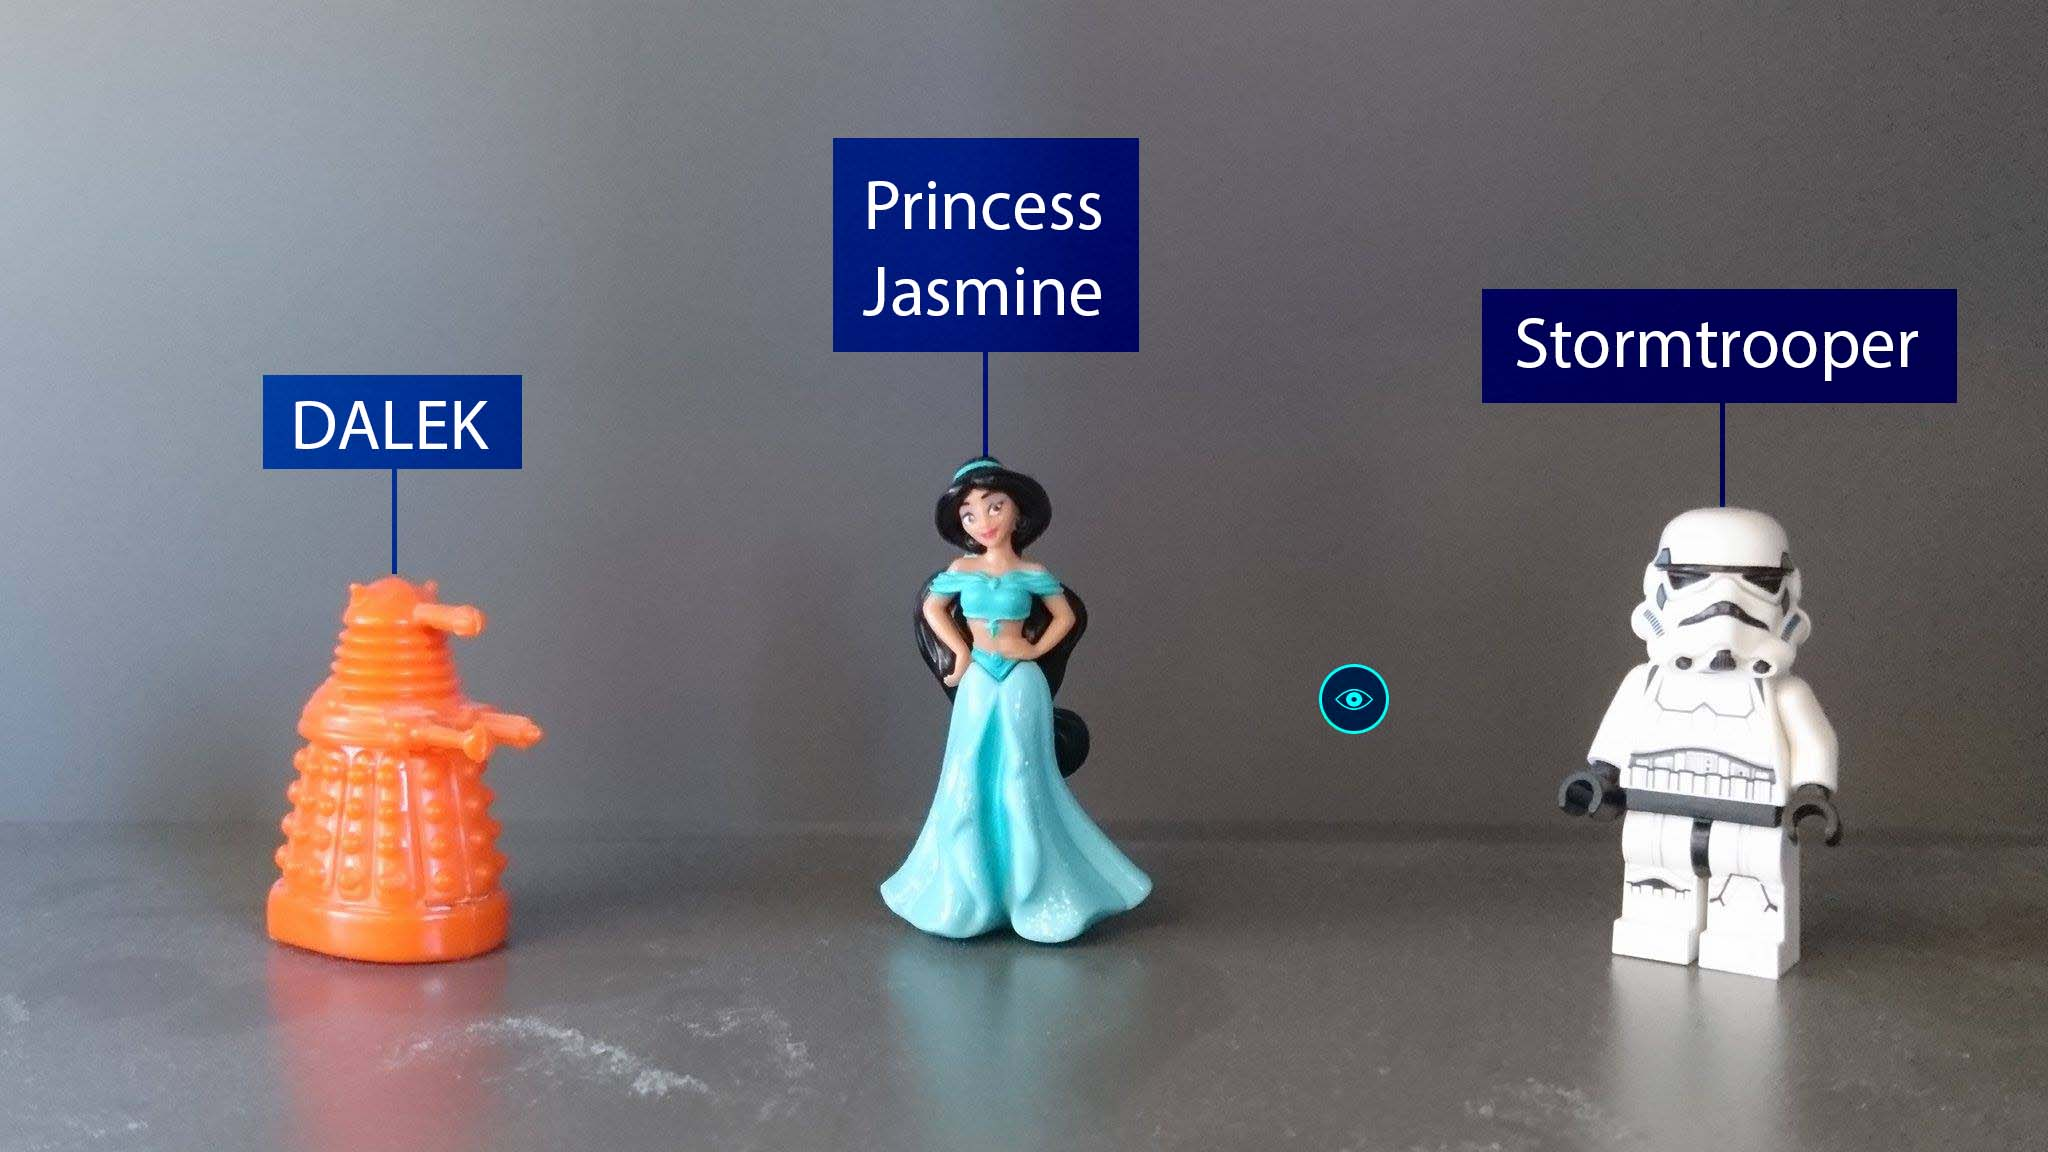
\includegraphics[width=0.5\textwidth]{Images/infoActive.jpg}
    	\caption{Condition where information is visible at all times (non-retrieval condition)
}
\end{figure}

\begin{figure}[htbp]
		\hspace{0.25\textwidth}
        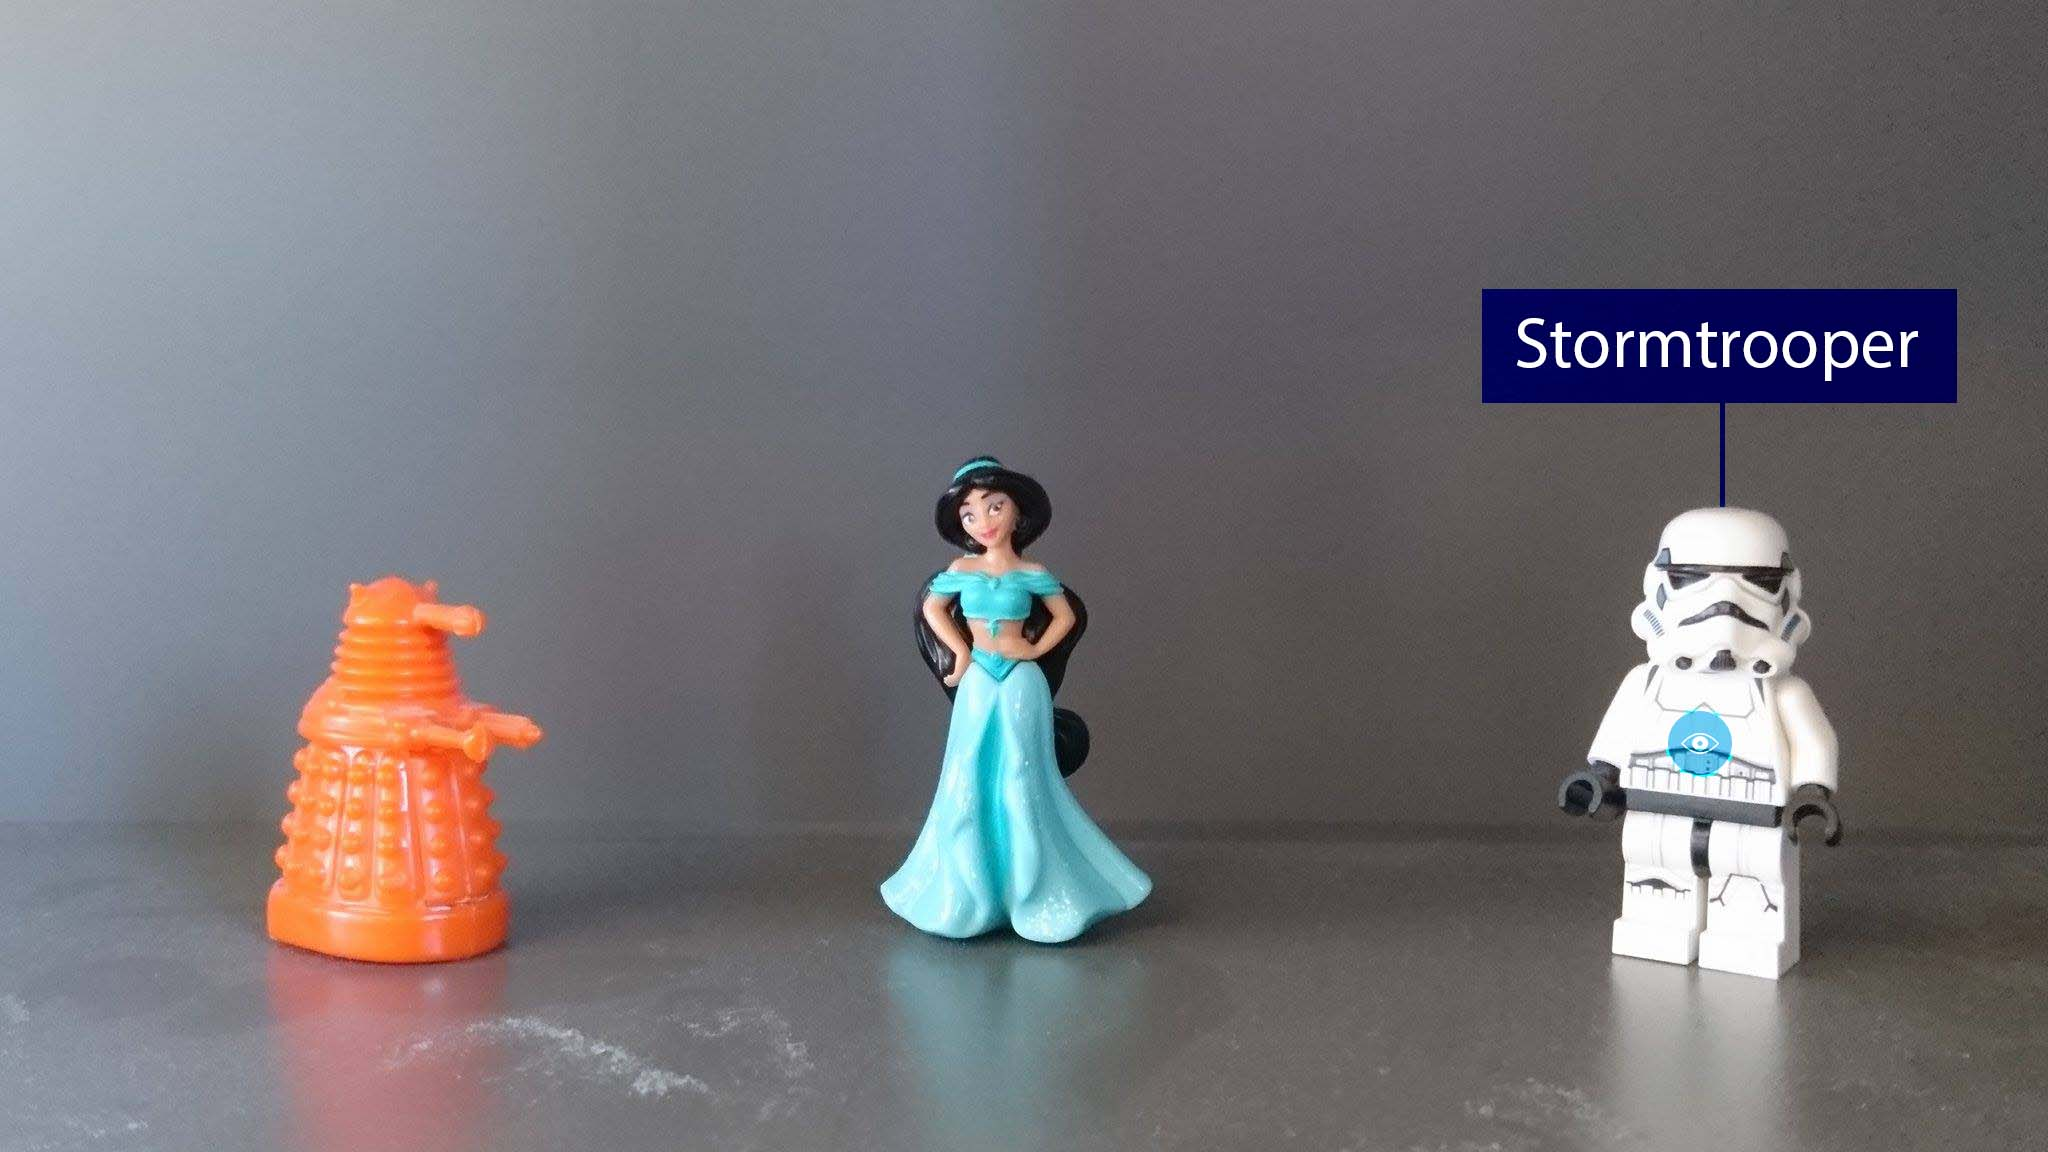
\includegraphics[width=0.5\textwidth]{Images/infoPassive.jpg}
    	\caption{Condition where information is visible only on when gazed upon (retrieval condition)
}
\end{figure}

The fact that overlays are not visible all the time solves the issue of occlusion (labels hiding other labels and labels hiding other objects in the scene). However, in this model the user is given no indication that there is gaze driven information present. This is a problem especially when there is a mixture of objects with and without associated information in the environment. It is for this reason that the second variable being investigated is the use of object outline cues or strokes. 

\subsection{Object Outline Cues}
As mentioned earlier another aim of this study is to investigate the impact of object outline cues on mental effort investment, information retention, and task performance. I intend to use a stroke around any object that has information retrievable associated information, thus differentiating between objects with and without associated data. In order to do this, the experimental design of the study must compare conditions where strokes are not used on objects (Figure 17), strokes are always visible (Figure 18) and strokes are visible if a user's gaze sweeps across the object (Figure 19).  

\begin{figure}[htbp]
		\vspace{0.35cm}
		\hspace{0.25\textwidth}
        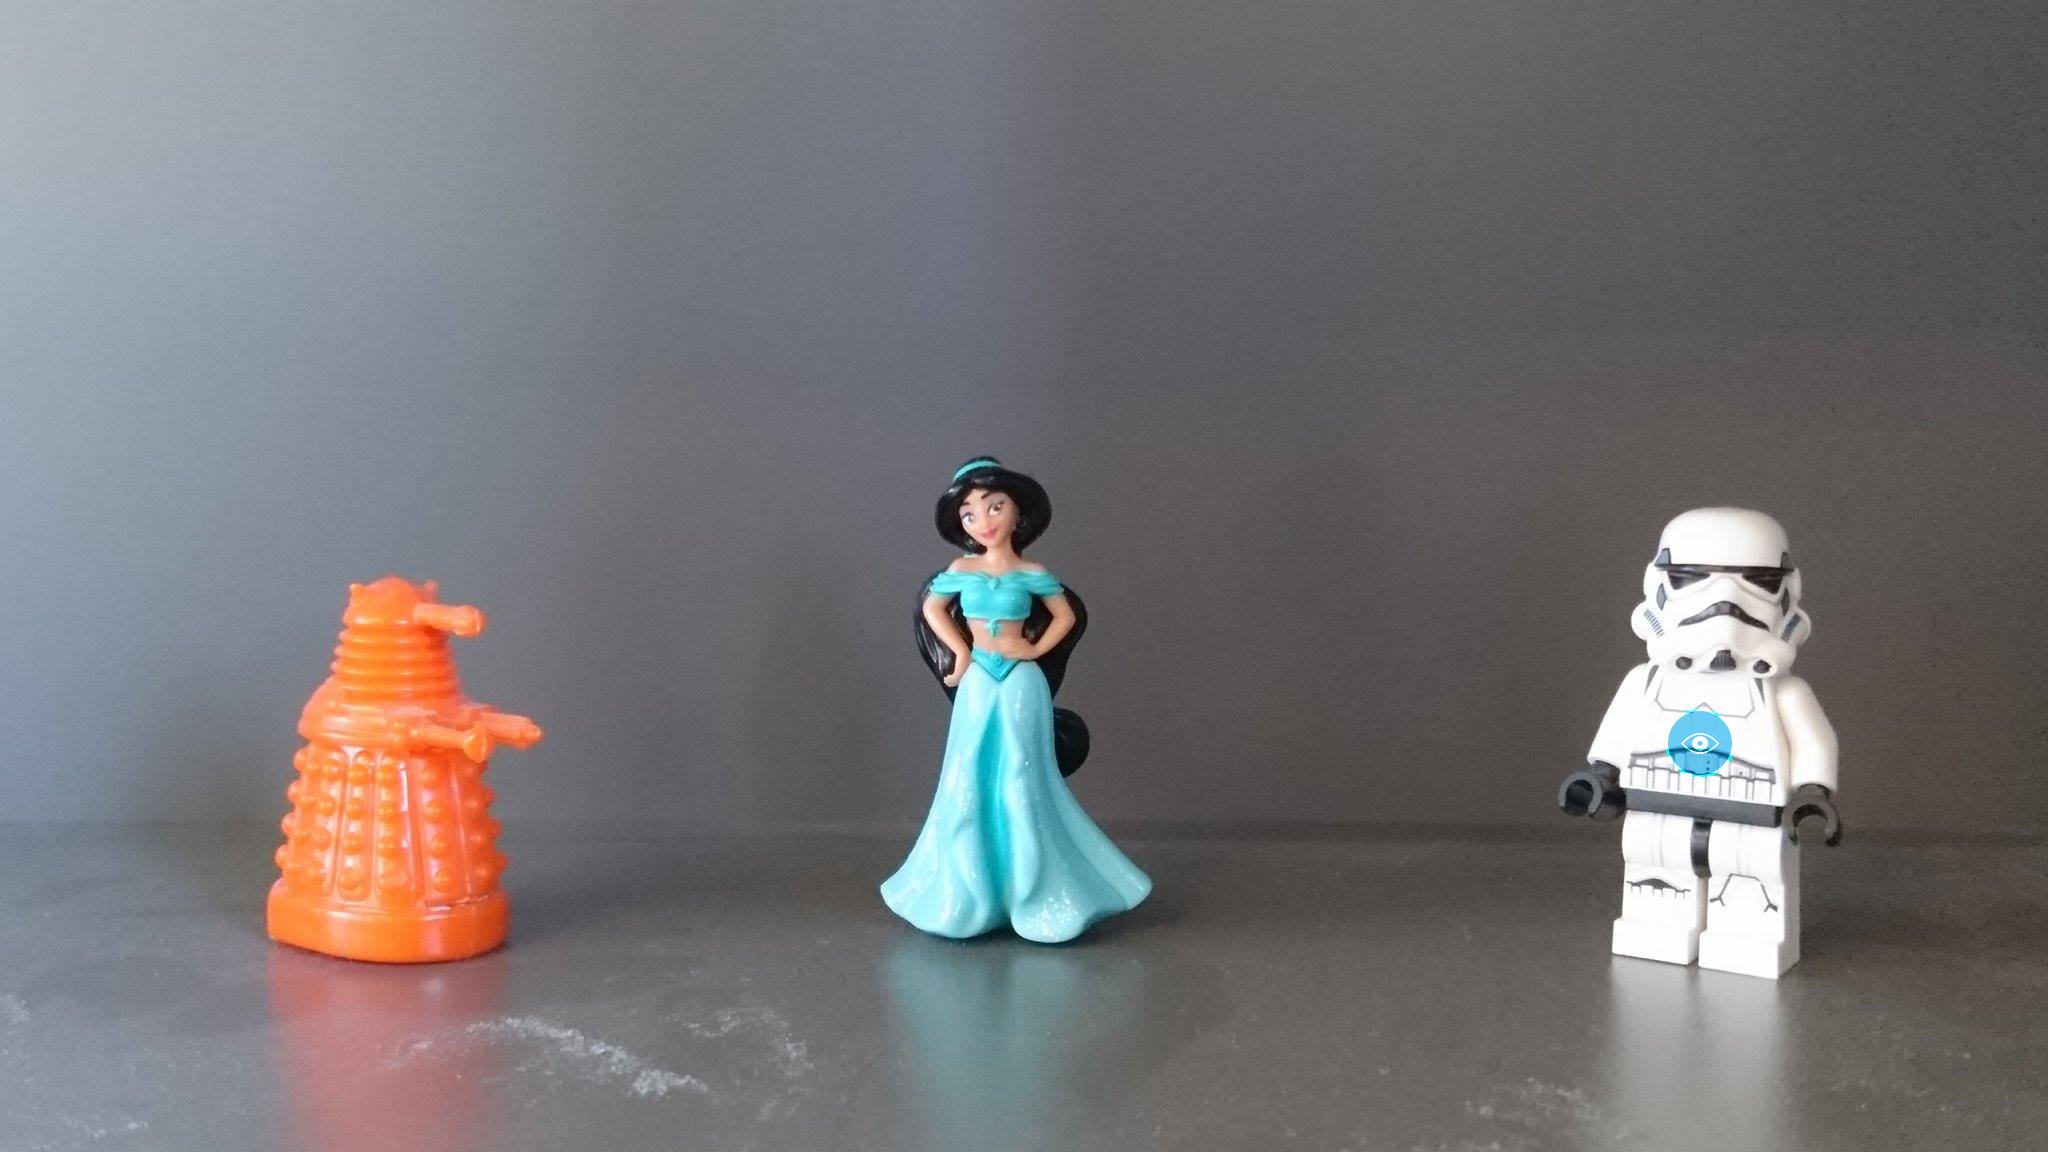
\includegraphics[width=0.5\textwidth]{Images/oultlineNone.jpg}
    	\caption{Outlines are not used. No changes when user gazes on objects or not. 
        \vspace{0.35cm}
}
\end{figure}

\begin{figure}[htbp]
		\hspace{0.25\textwidth}
        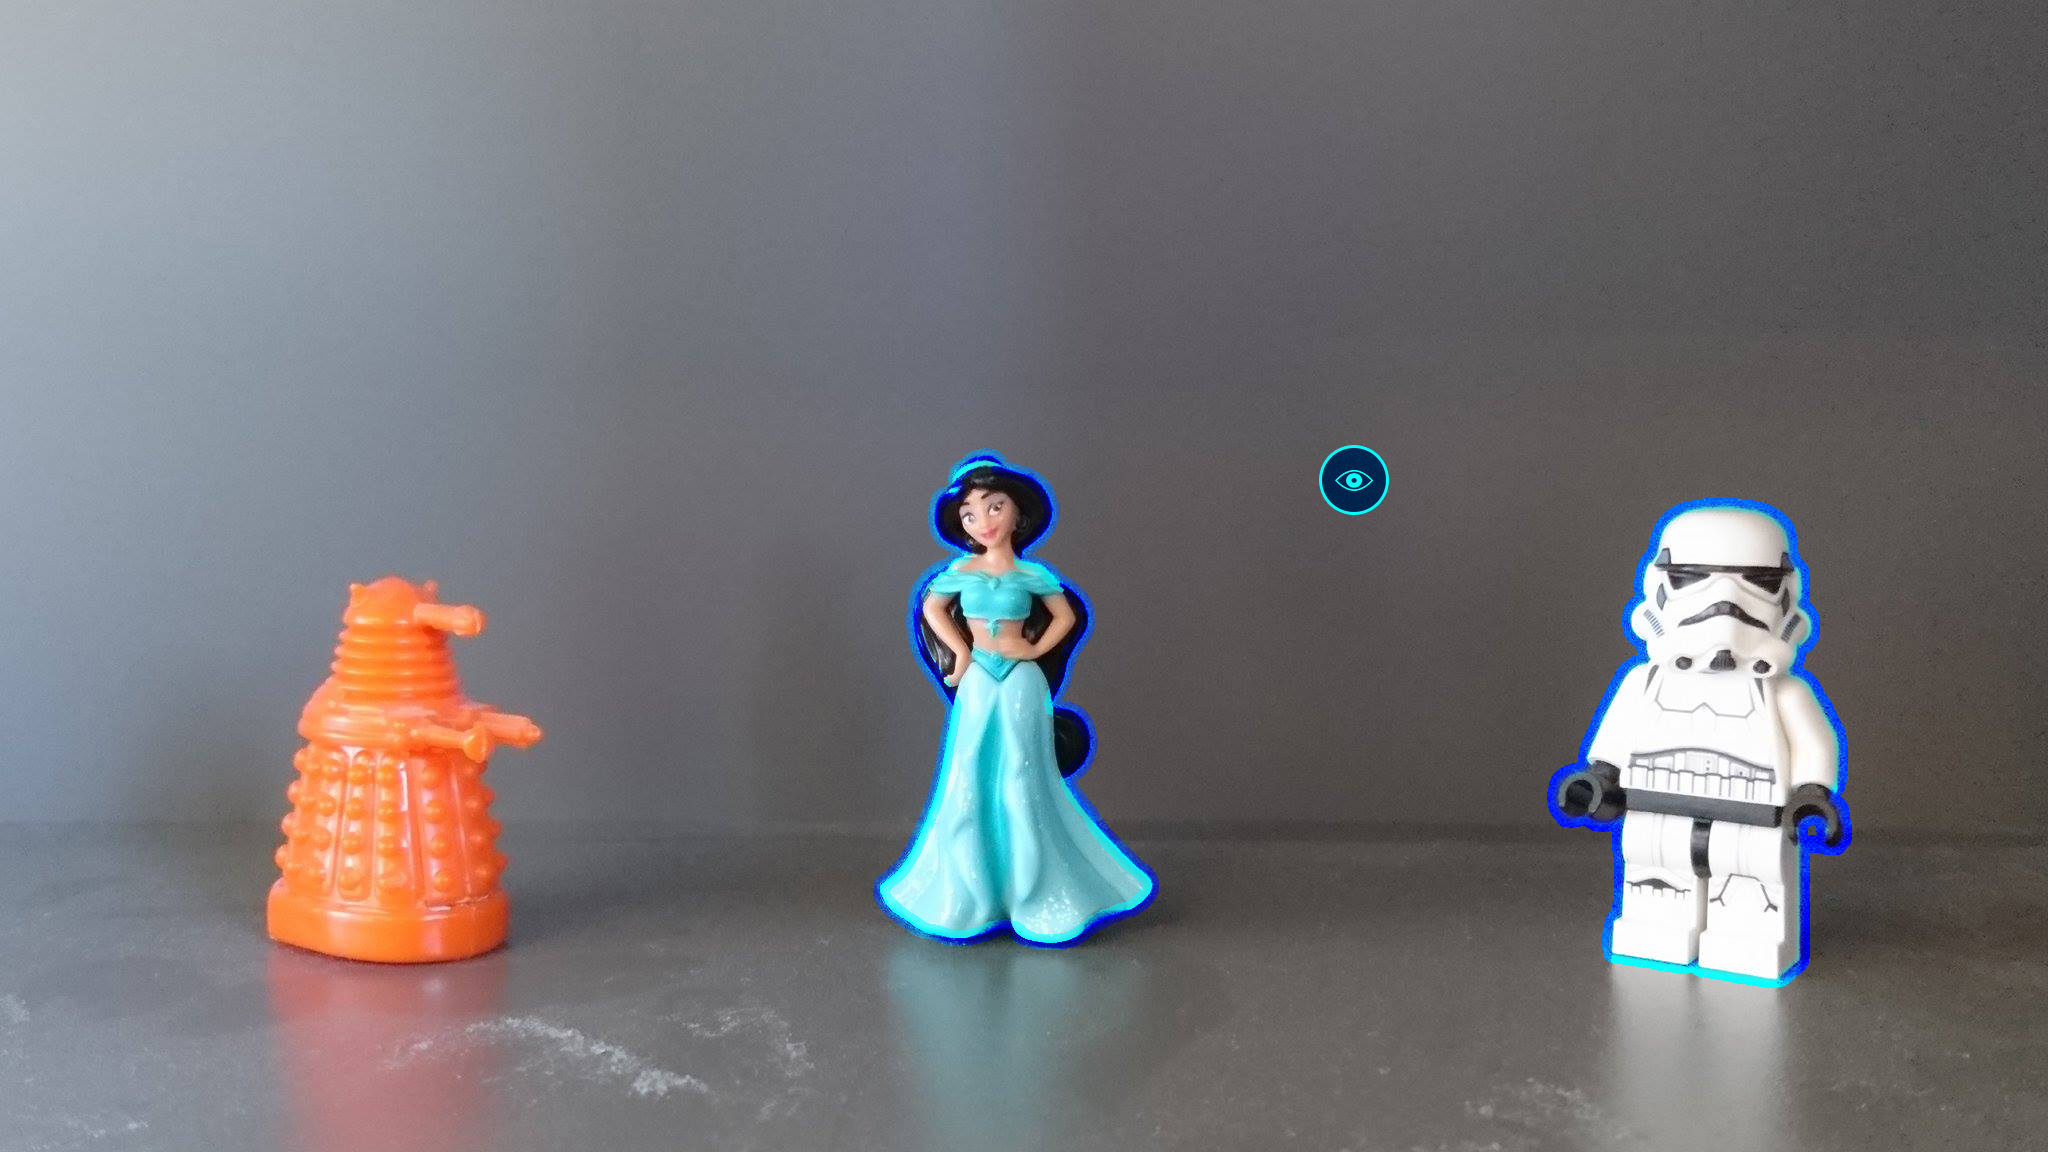
\includegraphics[width=0.5\textwidth]{Images/oultlineActive.jpg}
    	\caption{Outlines are always on, indicating objects in the scene users can retrieve information from.
}
\end{figure}

\begin{figure}[htbp]
		\hspace{0.25\textwidth}
        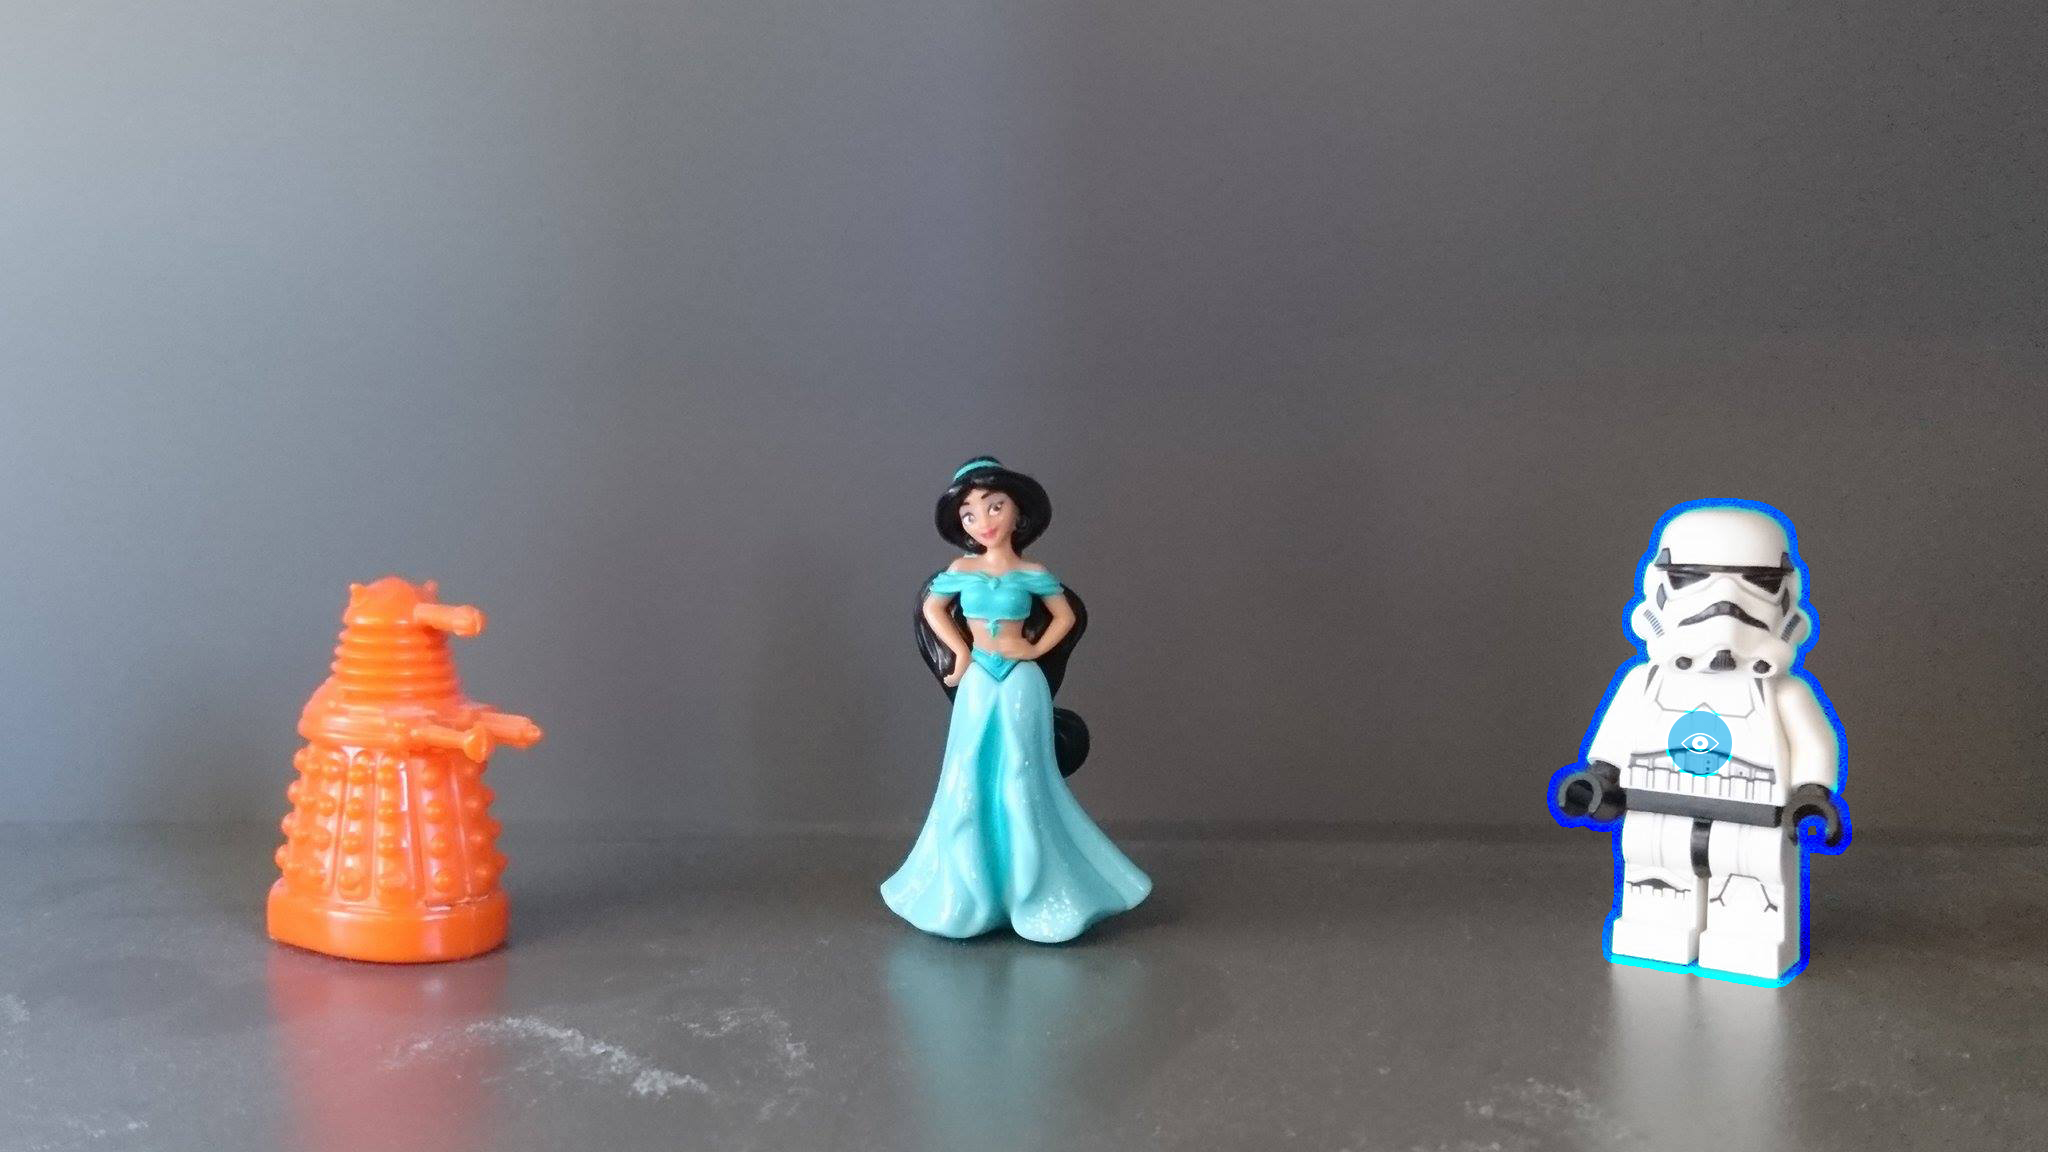
\includegraphics[width=0.5\textwidth]{Images/oultlineGaze.jpg}
    	\caption{As the user's gaze sweeps across object, the outlines are activated.
}
\end{figure}

It is important to note that the conditions shown in figures 18 and 19 are similar to each other. The difference is, that strokes being activated by user-gaze (figure 19) preserve the naturalness of the scene and force users to visually engage with the scene more (potentially increasing their mental effort investment). Also, since gaze is used both to indicate object strokes and for information retrieval, in a condition where both effects are being tested together, a delay would be needed before information is presented. For instance if a user gazes on an object, the stroke would appear immediately and if the gaze remains on the object for a set length of time (to be determined) the information about the object is retrieved.

I have designed a controlled experiment describing the effect of the variables described above and their impact on information retention, mental load and task performance, which I will now describe.

\section{Experimental Design} \label{Evidence}
The experimental design tests the individual conditions of the variables described above and the interaction between the two variables. The various conditions are described below:
\begin{itemize}
\item The conditions for the Information Retrieval variable are: 
	\begin{enumerate}
	\item The information is always visible, non-retrieval condition: $IR^{ off}$
    \item The information must be retrieved by the user through the gaze interaction: $IR^{ on}$ 
	\end{enumerate}
\item The conditions for the Stroke variable are:
	\begin{enumerate}
	\item The Stroke is not used: $S^{ off}$
    \item The Stroke is always on: $S^{ on}$
    \item The Stroke is activated by the user's gaze: $S^{ gaze}$
	\end{enumerate}
\end{itemize}
Table 1 shows the possible conditions the experimental design incorporates to test the variables and any interaction effect between the two. The experiment follows a $2\times3$ design. 

\captionof{table}{Experimental Design Conditions} \label{tab:title} 
{\renewcommand{\arraystretch}{2}%
\begin{tabular}{ C{0.1\textwidth} | C{0.375\textwidth} | C{0.375\textwidth}}\toprule[1.5pt]
 & \bf $IR^{ off}$ & \bf  $IR^{ on}$ \\
\hline
\bf $S^{ off}$        &\cellcolor{blue!8}  $C^1$: No stroke is used and information about the object is always on    &\cellcolor{blue!8}  $C^2$: No Stroke is used, user must retrieve information using gaze\\  
\hline
\bf $S^{ on}$        &  $C^3$: Stroke is used and information about the object is always visible     &\cellcolor{blue!8}  $C^4$: Stroke is always visible, user must retrieve information about the object using gaze\\
\hline
\bf $S^{ gaze}$        &  $C^5$: Stroke is triggered on gaze and information about the object is always visible, \bf this is a redundant condition and will not be tested     & $C^6:$ The stroke is triggered on gaze and if the gaze persists, the information is retrieved\\
\hline
\end {tabular}\par
\bigskip

From the table we can further eliminate other redundancies. Conditions $C^1$ and $C^3$ are testing similar effects since no information retrieval is required the user will always have access to object information so the strokes indicating the possibility of information retrieval is redundant.For the purposes of this study $C^1$ will be used where no stroke is used but information is present in view at all times.

There is considerable similarity between conditions $C^4$ and $C^6$ as well. Condition $C^6$ can be considered a situation where the effect of the Stroke is minimized to force the user to visually engage with the scene further. It is possible that the method could have an impact on information retention, mental effort investment and task performance. However, since this work has not been addressed by previous research it could be more effective to first test the effect in a condition such as $C^4$ which is an extreme application of the stroke effect. If using the stroke has a significant impact on the dependent variables, conditions $C^4$ and $C^6$ can be compared in  a follow up study.

In table 1, the cells that have been shaded blue will be tested in the experiment.

In summary, the independent variables in my study are Information Retrieval and Object Strokes and the dependent variables are Information Retention, Mental Effort Investment and Task Performance. For the purposes of the initial exploration study, the following conditions will be tested:
\begin{itemize}
\item $C^1$: No stroke and information about the object is always ON. This could be considered as the control condition.
\item $C^2$: No Stroke is used and users will have to retrieve information using gaze. This condition would test the effect of information retrieval on the dependent variables. 
\item $C^4$: The stroke is always on and users will have to retrieve information about the object using gaze. This condition would test the effect stroke has in supporting information retrieval on the dependent variables. 
\end{itemize}
I suggest investigating $C^6$ (gaze-triggered stroke and gaze-triggered data overlays) in a follow up study.

\section{Supporting Evidence} \label{Evidence}
Past research (see section 2) leads me to expect that using object outlines and user-driven information retrieval could have a meaningful  effect on mental cognition. The study conducted by Fiorentino et al \cite{fiorentino2013augmented} showed that text presentation (in this case style) affected completion time and error rate of tasks. Since my study explores interaction models that directly affect the way text is presented to the user, I can expect my interaction model to also affect task performance.

I expect my user-driven information retrieval interaction model to require increased mental effort investment from the user and positively impact cognitive performance. Pashler \cite{pashler1998psychology} hypothesizes that as mental effort increases cognitive performance increases. This effect is observed in Salomon's study \cite{salomon1984television} comparing television and reading. Reading demanded more mental effort investment and resulted in better learning inference. The results of my experiment may support some aspects Salomons hypothesis.

It may be that the proposed interaction model does not have a significant impact on mental effort or information retention and all the alternatives tested prove to be just as viable. Those results would still be useful as there are significant implications to the production (like set design) phase of content generation especially in interactive 360 video, if all interaction models are equally viable. My study will also gather user preferences from participants to explore which of these techniques would be more acceptable to viewers, separate from any effect on task performance.

\section{Importance of Proposed Study} \label{Importance}
As suggested in the section above, results of this study could inform the production phase of virtual reality content for things like set design  and script writing. It also has implications in augmented reality applications. It would be essential to know the cognitive impact different interaction models have on viewers. Since receiving contextually relevant textual data (and potentially  multimedia data) about a scene using HMDs is relevant to both AR and VR applications this project would be useful to the media production industry, as well as, academic research in Human Computer Interaction and Computer Vision. 

It is also important to note that with the lower display resolution of present HMD technology, it is difficult to pick up rich sensory cues from 360 video, this technique could be used to complement objects in 360 video to provide viewers with additional content.  

In the context of user experience in 360 video Passmore et al \cite{passmore2016effects} conducted a study comparing viewing conditions of 360 video in a HMD, on a mobile device and on a regular television screen. They note: 

\textit{"Panoramic video seems particularly well suited to situations where the viewer can explore and look around at own their pace, much as they might do in a gallery, or a crowded market situation, where the experience is user led rather than led by a director."}\cite{passmore2016effects}

My interaction model complements the user led exploratory nature the authors refer to and this technique could be used to enhance the experience of viewing and interacting with 360 video.

It is also worth highlighting that the approach described above can be considered as a viable primary research activity that could be scalable in multiple directions depending on the initial results gathered. 

\section{Timeline for Study} \label{Timeline}
The timeline of the project has been broken down according to activities that would be undertaken on a monthly basis:
\begin{itemize}
\item May: Literature review and technical implementations of demos for testing
\item June: Wrap-up of implementation and beginning of experimental study with participants.
\item July: End of study (and potentially a second study depending on results from the first and available time). 
\item August: Wrap -up of study (first or second), data analysis and writing of project report.
\end{itemize}

\section{Requirements of the Project} \label{Requirements}
I will need to recruit participants for the study. The number of participants will vary depending in the experimental design (within or between designs, number of conditions) and number of studies conducted. At the moment for the first study outlined in this document about 25-30 participants could potentially be required to test for statistically significant effects. 

\section{Concluding Notes} \label{Conclusion}
The project proposed here would draw from a review of past research including text representation in HMDs, present applications, cognitive implications of mental effort investment, attention and memory. It will involve the prototyping of these techniques and the evaluation of these prototypes in controlled experiments. 

Since HMD technology is continuously evolving, having a framework of how to augment contextually relevant information in the scene is a non-hardware specific field of study that would be useful to future applications of AR and VR. 

\newpage
\bibliographystyle{plain}
\bibliography{bibliography.bib}
\end{document}
